% Phase 2 request flow per protocol layer (build: tectonic phase2_request_flow.tex)
\documentclass[border=8pt]{standalone}
\usepackage[T1]{fontenc}
\usepackage{lmodern}
\usepackage{tikz}
\usetikzlibrary{arrows.meta,calc}

\definecolor{dnsc}{HTML}{2E75B6}
\definecolor{edgec}{HTML}{C55A11}
\definecolor{appc}{HTML}{548235}
\definecolor{tlsc}{HTML}{7030A0}
\definecolor{fwc}{HTML}{C00000}

\tikzset{
  head/.style={draw, fill=gray!12, rounded corners=2pt, minimum width=2.5cm, minimum height=0.85cm,
               align=center, font=\footnotesize\bfseries},
  msg/.style={-{Stealth[length=2.2mm]}, line width=0.7pt, draw=#1},
  t/.style={font=\scriptsize, fill=white, inner sep=1pt, text=#1},
  layer/.style={font=\scriptsize\bfseries, text=#1, anchor=east, align=right},
}

\begin{document}
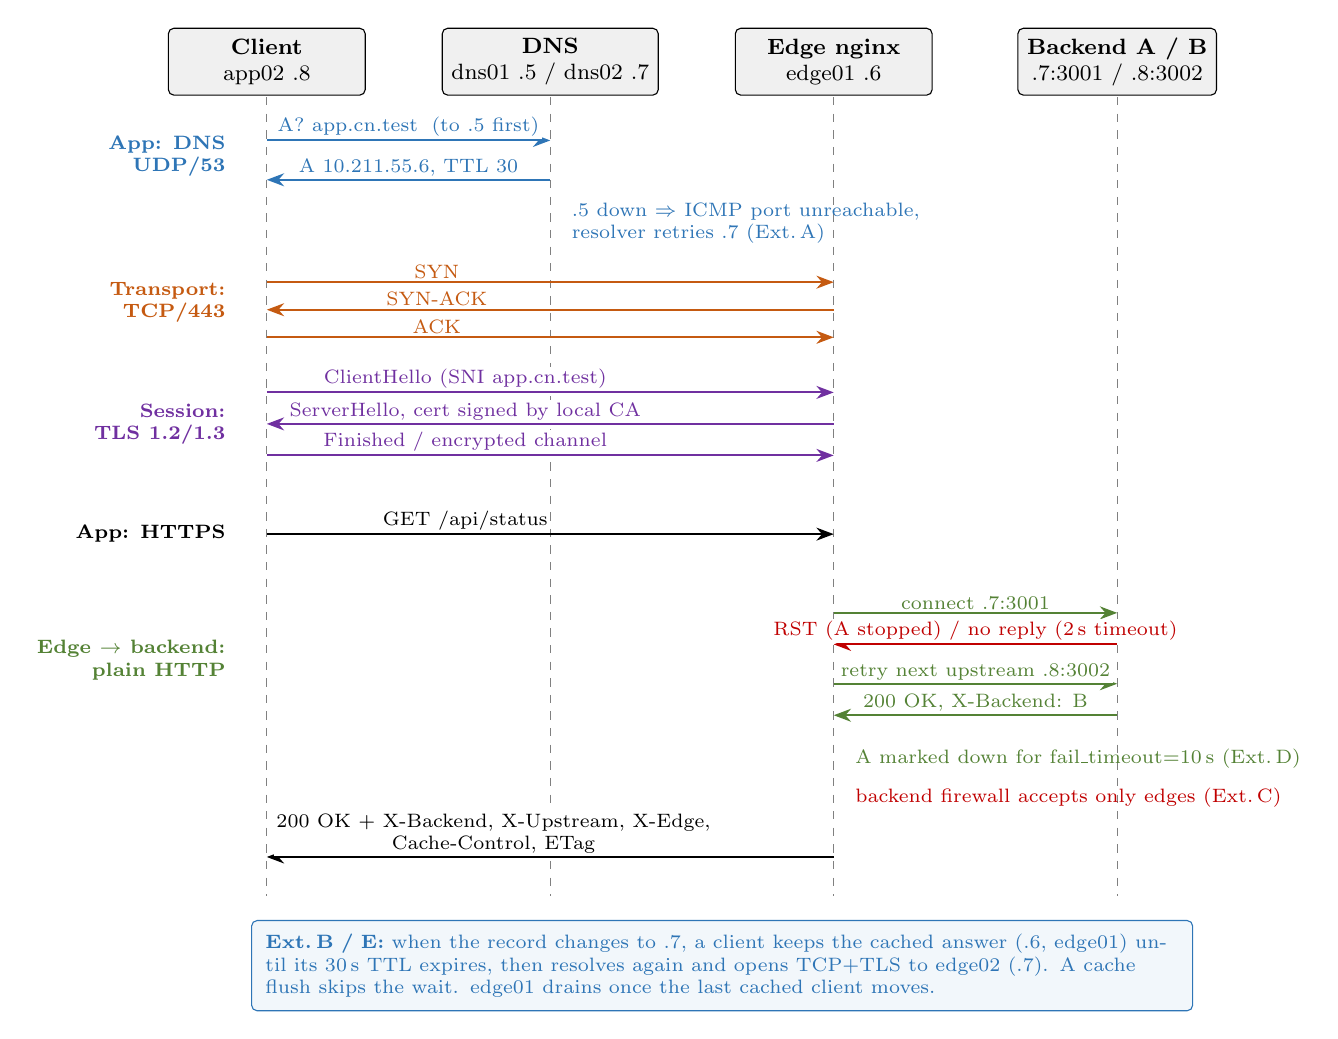
\begin{tikzpicture}
% lifeline x positions
\def\xC{0} \def\xD{3.6} \def\xE{7.2} \def\xA{10.8}
\node[head] (C) at (\xC,0) {Client\\\normalfont app02 .8};
\node[head] (D) at (\xD,0) {DNS\\\normalfont dns01 .5 / dns02 .7};
\node[head] (E) at (\xE,0) {Edge nginx\\\normalfont edge01 .6};
\node[head] (A) at (\xA,0) {Backend A / B\\\normalfont .7:3001 / .8:3002};
\foreach \x in {\xC,\xD,\xE,\xA} \draw[gray, dashed] (\x,-0.45) -- (\x,-10.6);

% ---- L7 DNS
\node[layer=dnsc] at (-0.4,-1.2) {App: DNS\\UDP/53};
\draw[msg=dnsc] (\xC,-1.0) -- node[t=dnsc, above] {A? app.cn.test \;(to .5 first)} (\xD,-1.0);
\draw[msg=dnsc] (\xD,-1.5) -- node[t=dnsc, above] {A 10.211.55.6, TTL 30} (\xC,-1.5);
\node[font=\scriptsize, text=dnsc, align=left, anchor=west] at (\xD+0.15,-2.05)
  {.5 down $\Rightarrow$ ICMP port unreachable,\\ resolver retries .7 (Ext.\,A)};

% ---- L4 TCP
\node[layer=edgec] at (-0.4,-3.05) {Transport:\\TCP/443};
\draw[msg=edgec] (\xC,-2.8) -- node[t=edgec, above, pos=0.3] {SYN} (\xE,-2.8);
\draw[msg=edgec] (\xE,-3.15) -- node[t=edgec, above, pos=0.7] {SYN-ACK} (\xC,-3.15);
\draw[msg=edgec] (\xC,-3.5) -- node[t=edgec, above, pos=0.3] {ACK} (\xE,-3.5);

% ---- TLS
\node[layer=tlsc] at (-0.4,-4.6) {Session:\\TLS 1.2/1.3};
\draw[msg=tlsc] (\xC,-4.2) -- node[t=tlsc, above, pos=0.35] {ClientHello (SNI app.cn.test)} (\xE,-4.2);
\draw[msg=tlsc] (\xE,-4.6) -- node[t=tlsc, above, pos=0.65] {ServerHello, cert signed by local CA} (\xC,-4.6);
\draw[msg=tlsc] (\xC,-5.0) -- node[t=tlsc, above, pos=0.35] {Finished / encrypted channel} (\xE,-5.0);

% ---- HTTP to edge
\node[layer=black] at (-0.4,-6.0) {App: HTTPS};
\draw[msg=black] (\xC,-6.0) -- node[t=black, above, pos=0.35] {GET /api/status} (\xE,-6.0);

% ---- behind edge
\node[layer=appc] at (-0.4,-7.6) {Edge $\to$ backend:\\plain HTTP};
\draw[msg=appc] (\xE,-7.0) -- node[t=appc, above] {connect .7:3001} (\xA,-7.0);
\draw[msg=fwc] (\xA,-7.4) -- node[t=fwc, above] {RST (A stopped) / no reply (2\,s timeout)} (\xE,-7.4);
\draw[msg=appc] (\xE,-7.9) -- node[t=appc, above] {retry next upstream .8:3002} (\xA,-7.9);
\draw[msg=appc] (\xA,-8.3) -- node[t=appc, above] {200 OK, X-Backend: B} (\xE,-8.3);
\node[font=\scriptsize, text=appc, align=left, anchor=west] at (\xE+0.15,-8.85)
  {A marked down for fail\_timeout=10\,s (Ext.\,D)};
\node[font=\scriptsize, text=fwc, align=left, anchor=west] at (\xE+0.15,-9.35)
  {backend firewall accepts only edges (Ext.\,C)};

% ---- response
\draw[msg=black] (\xE,-10.1) -- node[t=black, above, pos=0.6, align=center] {200 OK + X-Backend, X-Upstream, X-Edge,\\ Cache-Control, ETag} (\xC,-10.1);

% ---- cutover note
\node[draw=dnsc, rounded corners=2pt, fill=dnsc!6, font=\scriptsize, text=dnsc, align=left, text width=11.6cm, inner sep=5pt, anchor=north west] at (\xC-0.2,-10.9)
  {\textbf{Ext.\,B / E:} when the record changes to .7, a client keeps the cached answer (.6, edge01) until its 30\,s TTL expires, then resolves again and opens TCP+TLS to edge02 (.7). A cache flush skips the wait. edge01 drains once the last cached client moves.};
\end{tikzpicture}
\end{document}
